% !TeX program = pdflatex
\documentclass[tikz,border=8pt]{standalone}
\usepackage{tikz}
\usetikzlibrary{angles,quotes,positioning}
\definecolor{FigureBlue}{HTML}{2563EB}
\definecolor{FigureOrange}{HTML}{EA580C}
\definecolor{FigureSlate}{HTML}{64748B}
\begin{document}
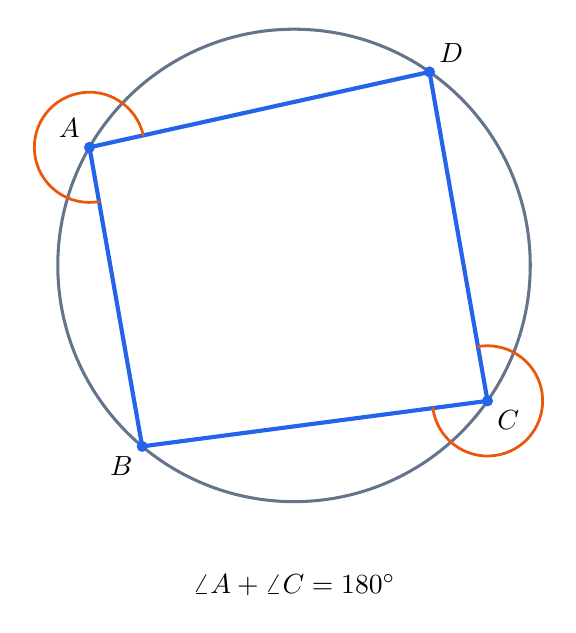
\begin{tikzpicture}[line cap=round,line join=round]
  \coordinate (O) at (0,0);
  \coordinate (A) at (150:3);\coordinate (B) at (230:3);\coordinate (C) at (325:3);\coordinate (D) at (55:3);
  \draw[FigureSlate,line width=1.1pt] (O) circle[radius=3];
  \draw[FigureBlue,line width=1.5pt] (A)--(B)--(C)--(D)--cycle;
  \pic[draw=FigureOrange,line width=1pt,angle radius=7mm] {angle=D--A--B};
  \pic[draw=FigureOrange,line width=1pt,angle radius=7mm] {angle=B--C--D};
  \foreach \P in {A,B,C,D}{\fill[FigureBlue] (\P) circle (2pt);}
  \node[above left] at (A) {$A$};\node[below left] at (B) {$B$};\node[below right] at (C) {$C$};\node[above right] at (D) {$D$};
  \node[below=8mm] at (0,-3) {$\angle A+\angle C=180^{\circ}$};
\end{tikzpicture}
\end{document}
